\documentclass[11pt]{article}
\usepackage[a4paper,margin=2.2cm]{geometry}
\usepackage[T1]{fontenc}
\usepackage{tgpagella,mathpazo,booktabs,longtable,array,microtype}
\usepackage[scaled=.95]{helvet}
\usepackage[dvipsnames,table]{xcolor}
\usepackage{tikz}
\usetikzlibrary{arrows.meta,positioning}
\usepackage[hidelinks]{hyperref}
% Shared manuscript and TikZ visual language for the OPERA paper.
% Keep colours and Helvetica-like figure typography synchronized with
% opera/visualization/style.py (Arial/Liberation Sans on render hosts).

\definecolor{OperaIndigo}{HTML}{2D3A8C}
\definecolor{OperaNavy}{HTML}{1A237E}
\definecolor{OperaPeriwinkle}{HTML}{5C7AEA}
\definecolor{OperaSlate}{HTML}{737D8C}
\definecolor{OperaTeal}{HTML}{408579}
\definecolor{OperaGreen}{HTML}{1B7A4A}
\definecolor{OperaSienna}{HTML}{B5451B}
\definecolor{OperaTerracotta}{HTML}{C16A58}
\definecolor{OperaOchre}{HTML}{B18B4D}
\definecolor{OperaLavender}{HTML}{8974AC}
\definecolor{OperaInk}{HTML}{17212B}
\definecolor{OperaInkSecondary}{HTML}{485463}
\definecolor{OperaInkMuted}{HTML}{657180}
\definecolor{OperaBorder}{HTML}{CBD2DA}
\definecolor{OperaGrid}{HTML}{E8ECF1}
\definecolor{OperaPaper}{HTML}{F7F8FA}

\tikzset{
  opera/.style={font=\sffamily\small, text=OperaInk},
  panel/.style={draw=none, fill=white, inner sep=0pt},
  softpanel/.style={
    rounded corners=0.8mm,
    draw=OperaGrid,
    line width=0.45pt,
    fill=OperaPaper,
    inner sep=2.4mm,
  },
  stage/.style={
    rounded corners=0.7mm,
    draw=OperaBorder,
    line width=0.6pt,
    fill=white,
    align=center,
    minimum height=8mm,
    inner xsep=3mm,
    inner ysep=1.8mm,
  },
  stageblue/.style={stage, draw=OperaIndigo!55, fill=OperaIndigo!7},
  stageteal/.style={stage, draw=OperaTeal!65, fill=OperaTeal!8},
  stagewarm/.style={stage, draw=OperaSienna!60, fill=OperaSienna!7},
  latent/.style={
    circle,
    draw=OperaIndigo!65,
    fill=OperaIndigo!9,
    line width=0.6pt,
    minimum size=6mm,
    inner sep=0pt,
    font=\sffamily\scriptsize\bfseries,
  },
  token/.style={
    rounded corners=0.7mm,
    draw=OperaBorder,
    fill=white,
    minimum width=6.2mm,
    minimum height=4.8mm,
    inner sep=0.5mm,
    font=\sffamily\tiny,
    align=center,
  },
  outcome/.style={
    rounded corners=1mm,
    draw=OperaTerracotta!70,
    fill=OperaTerracotta!9,
    minimum height=5.8mm,
    inner xsep=1.8mm,
    font=\sffamily\scriptsize,
    align=center,
  },
  flow/.style={
    -{Latex[length=2mm,width=1.2mm]},
    line width=0.75pt,
    draw=OperaInkSecondary,
  },
  flowblue/.style={flow, draw=OperaIndigo},
  flowteal/.style={flow, draw=OperaTeal},
  flowwarm/.style={flow, draw=OperaSienna},
  relation/.style={
    -{Latex[length=1.8mm,width=1.1mm]},
    line width=0.65pt,
    draw=OperaLavender,
    densely dashed,
  },
  captionnote/.style={
    font=\sffamily\fontsize{6.6}{7.5}\selectfont,
    text=OperaInkMuted,
    align=center,
  },
  labelsmall/.style={
    font=\sffamily\fontsize{7}{8}\selectfont,
    text=OperaInkSecondary,
    align=center,
  },
  heading/.style={
    font=\sffamily\fontsize{9}{10}\selectfont\bfseries,
    text=OperaInk,
    align=left,
  },
  panelletter/.style={font=\sffamily\bfseries\normalsize, text=OperaInk},
  divider/.style={draw=OperaBorder, line width=0.45pt},
  eyebrow/.style={font=\sffamily\fontsize{6.5}{7.5}\selectfont\bfseries,
    text=OperaIndigo, align=left},
}

\setlength{\parindent}{0pt}
\setlength{\parskip}{6pt}
\renewcommand{\arraystretch}{1.2}
\renewcommand{\thetable}{M\arabic{table}}
\newcolumntype{L}[1]{>{\raggedright\arraybackslash}p{#1}}
\newcommand{\pending}{\textcolor{OperaSienna}{Pending artifact audit}}
\begin{document}
\ifdefined\embeddedSupplement\pagestyle{empty}\fi
\section*{Supplementary Methods: model development and evaluation}
Model development separates the origin of the patient representation from the
supervised information used to adapt it. The following sections describe these
components and their evaluation. Tables distinguish the confirmed local
specification from details awaiting completed-run verification; empirical
performance remains to be inserted from the locked analyses.
\tableofcontents

\section{Transformer and prediction architecture}
Chronological patient histories are encoded by a causal transformer. A common
encoder initialization is used across supervision scopes so that their
comparison changes labelled experience rather than the starting representation.
Outcome heads convert interval hazards to cumulative incidence at the six
evaluation horizons. The local specification is summarised below.
\begin{longtable}{L{3.5cm}L{5.2cm}L{5.5cm}}
\caption{Local architecture specification and audit source.}\\
\toprule Setting & Current specification & Evidence required\\\midrule\endhead
Hidden width / layers / heads & 256 / 4 / 4 & Confirmed running specification; saved checkpoint audit pending\\
Temporal encoding & Scaled Time2Vec & Exact implementation, dimensions and units\\
Maximum context & 8,192 tokens & Resolved config and window/truncation policy\\
Feed-forward width / activation & \pending & Saved config and model module\\
Normalization / dropout / biases & \pending & Per-block and embedding settings\\
Vocabulary / numeric tokens & Frozen local vocabulary; joined-bin numeric tokens & Size/hash, fitted training view and bin metadata\\
Attention / padding / pooling & \pending & Mask semantics and patient readout\\
Hazard heads / causes & Interval hazards; primary and competing causes where applicable & Interval grids, head dimensions and CIF implementation\\
Objective & Known-status multi-horizon BCE & Grade/group weights and censoring masks\\
Router & Policy lock pending & Bank, rank, query width/mode, anchoring, scale, floors, shrinkage and initialization\\
Parameters & \pending & Total/trainable encoder, head and bank counts\\\bottomrule
\end{longtable}
Nation-scale encoder architecture must be reported separately; do not fill its fields with
local values. Record its source population, objective, vocabulary, temporal
encoding, dimensions and available budget provenance.

\section{Training phases and checkpoint selection}
Self-supervised fitting learns from pre-cutoff histories before outcome fitting.
The direct nation-scale arm performs vocabulary alignment without local
continuation; the adapted arm adds that continuation from the same artifact.
Supervised checkpoints are selected on the complete tuning set. Actual steps,
exposure and selected epochs will accompany the planned budgets below.
\begin{longtable}{L{2.4cm}L{5.5cm}L{6.3cm}}
\caption{Phase-specific training record.}\\
\toprule Phase & Starting point / scope & Final reporting fields\\\midrule\endhead
Local SSL & Local histories before 2022; confirmed 20-epoch running budget & Optimizer/schedule, batch/accumulation, precision, actual epochs/steps/tokens, selected checkpoint and hash\\
Nation-scale direct & Encoder-only export and vocabulary remapping & Source hash, overlap, local-only row initialization; no local SSL step\\
Local DAPT & Same direct nation-scale export; planned 20 epochs & Actual optimizer/batch/steps/tokens, source/selected hashes and checkpoint selection\\
Supervised S/D/O/J & Same local initializer; planned 30 epochs, seed 42 & Scope, exposure, natural sampling, full tuning BCE selection, actual epochs and selected epoch\\
Routed fits & Same supervision as J; tuning-locked policy & Matched training settings, bank/capacity policy and actual parameter counts\\
Tabular fits & Per disease/outcome/horizon & Feature recipe, search space/budget, log-loss tuning, final parameters and seeds\\\bottomrule
\end{longtable}
Record learning rate, warmup, weight decay, clipping, effective batch, validation
coverage, stopping/resume rules and hardware for every fit. Planned epochs are
not evidence of completed training or matched compute.

\section{Encoder origin and adaptation schematic}
\begin{center}
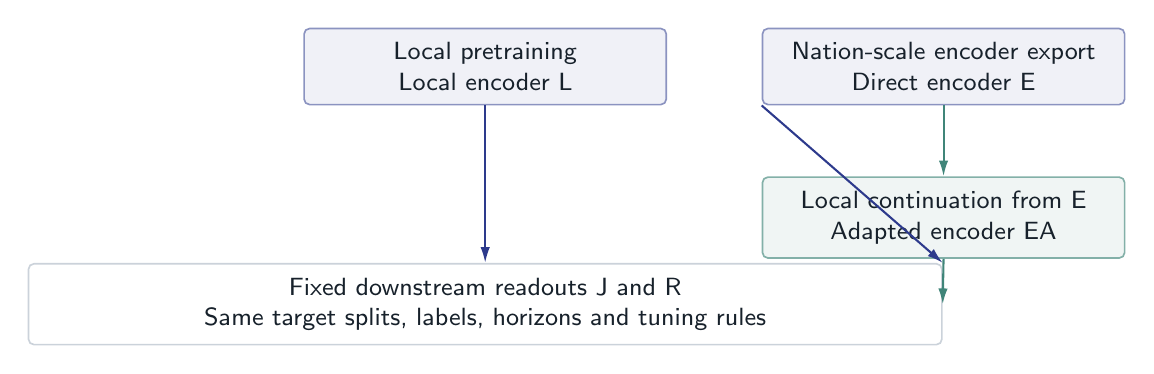
\begin{tikzpicture}[opera,node distance=9mm and 12mm]
\node[stageblue,text width=4cm] (l) {Local pretraining\\Local encoder L};
\node[stageblue,text width=4cm,right=of l] (e) {Nation-scale encoder export\\Direct encoder E};
\node[stageteal,text width=4cm,below=of e] (ea) {Local continuation from E\\Adapted encoder EA};
\draw[flowteal] (e)--(ea);
\node[stage,text width=11cm,below=20mm of l] (fits) {Fixed downstream readouts J and R\\Same target splits, labels, horizons and tuning rules};
\draw[flowblue] (l)--(fits);
\draw[flowblue] (e.south west)--(fits.north east);
\draw[flowteal] (ea.south)--(fits.east);
\end{tikzpicture}
\end{center}
Compare E--L, EA--E and EA--L separately for J/R. Report architecture and budget
mismatches explicitly. The selected router is not reselected on held-out data.

\section{Comparison with disease-specific prognostic indices}
Clinical-score comparisons are defined separately for each score, applicable
population, endpoint and horizon. Both systems are evaluated on identical
score-available patients with baseline information. The neural model produces
continuous risk; its groups use cutoffs fixed on tuning data. Original clinical
categories remain intact, so similarly named groups from different indices
are not pooled. The reporting fields below make those comparisons explicit.
\begin{longtable}{L{4cm}L{10.2cm}}
\caption{Fields required for every clinical-score comparison.}\\
\toprule Field & Required entry\\\midrule\endhead
Score / applicable population & Original score name/version and intended disease/treatment population\\
Availability & Known at treatment start; eligible/scored N, missingness by split/year\\
Endpoint / horizon & Definition, competing cause and support at the chosen horizon\\
Model grouping & Tuning-locked cutoffs; low-risk comparability and meaningful-size rationale\\
Score grouping & Original categories and continuous/integer score where available\\
Matched evaluation & Identical score-available patients; group N/events, KM survival or AJ incidence and intervals\\
Operating point & Tuning threshold, achieved held-out specificity, recall, precision and count basis\\
Reclassification & Cross-classification, discordant-group outcomes, uncertainty and sparse-cell status\\\bottomrule
\end{longtable}
NCCN-IPI/DLBCL provides the focused main example. Other valid score/population
pairs receive a common summary table and supplementary risk-group panels when
support permits. Detailed scatter, age and operating-point panels are warranted
when they answer a prespecified question; they are not obligatory for every
score. Unsupported comparisons remain in the availability inventory.

\section{Performance reporting}
The CSV headers in \texttt{supplement\_templates/} define run inventory,
absolute performance, paired contrasts, clinical-score applicability and
risk-group estimates. They intentionally contain no synthetic result rows.
Never replace unavailable values with zero. Metric tables record their estimand
and uncertainty method; each model is a single training run, so intervals
describe patient sampling only.

\section{Reproducibility and provenance}
Final specifications are derived from resolved configurations and completed
run records. Locked prediction and reviewed aggregate artifacts are linked by
source hashes and code versions, preserving their provenance through analysis
and figure generation.
See \texttt{SUPPLEMENT\_CONTENTS\_PLAN.md} for coverage, robustness, calibration,
compute and diagnostic requirements. Table 1 remains a separate cohort-review
artifact and needs supervisor sign-off.
\end{document}
